\documentclass[12pt]{article}
\usepackage{lmodern}
\usepackage[T1]{fontenc}
\usepackage[portuges]{babel}
\usepackage[utf8]{inputenc}
\usepackage{a4}
\usepackage{textgreek}
\usepackage{epstopdf}
\usepackage{graphicx}
\usepackage{fancyvrb}
\usepackage{amsmath}
\usepackage{float}
\usepackage{listings}
%\renewcommand{\baselinestretch}{1.5}


\begin{document}

\begin{titlepage}

\newcommand{\HRule}{\rule{\linewidth}{0.5mm}} % Defines a new command for the horizontal lines, change thickness here

\center % Center everything on the page
    
%----------------------------------------------------------------------------------------
%	HEADING SECTIONS
%----------------------------------------------------------------------------------------

\textsc{\LARGE Universidade do Minho}\\[1.5cm] 
\textsc{\Large Mestrado Integrado em Engenharia Informática}\\[0.5cm] 
\textsc{\large Computação Gráfica}\\[0.5cm]

%----------------------------------------------------------------------------------------
%	TITLE SECTION
%----------------------------------------------------------------------------------------

\HRule \\[0.4cm]
{ \huge \bfseries Curvas, Superfícies Cúbicas e VBOs}\\[0.4cm] 
\HRule \\[1.5cm]
    
%----------------------------------------------------------------------------------------
%	AUTHOR SECTION
%----------------------------------------------------------------------------------------

\begin{minipage}{0.4\textwidth}
\begin{flushleft} \large
\emph{Grupo:}\\
Etienne Costa A76089 \\
Joana Cruz A76270 \\
Rafael Alves A72629 \\
Maurício Salgado A71407 \\
\end{flushleft}
\end{minipage}
~
\begin{minipage}{0.4\textwidth}
\begin{flushright} \large
\emph{Docente:} \\
António Ramires\\
\end{flushright}
\end{minipage}\\[2cm]

%----------------------------------------------------------------------------------------
%	DATE SECTION
%----------------------------------------------------------------------------------------

{\large \today}\\[2cm]

%----------------------------------------------------------------------------------------
%	LOGO SECTION
%----------------------------------------------------------------------------------------


\includegraphics[scale=0.3]{uminho}\\
    
%----------------------------------------------------------------------------------------

\vfill % Fill the rest of the page with whitespace

\end{titlepage}

\tableofcontents
\newpage
\section{Introdução}
O relatório apresentado diz respeito à terceira fase do projeto proposto no âmbito da unidade curricular de
Computação Gráfica. O trabalho desta fase consiste na ilustração de animações relativas a uma
translação ou rotação. Ambas as transformações, contrariamente à fase anterior, passam a ser 
efetuadas num determinado período de tempo, sendo também uma translação definida através de
uma curva de Catmull-Rom.
Para além do descrito anteriormente, foi adicionada uma nova primitiva gráfica(Teapot), sendo esta baseada em Bézier Patches.
Quanto aos VBOs estes foram explicados na fase anterior, dado que foram implementados nessa fase.
Neste relatório descreve-se detalhadamente cada uma das componentes da
terceira fase. Começa-se por descrever as novas funcionalidades dos dois programas, Generator e Engine, bem como 
o modo de utilização das mesmas.
\newpage
\section{Gerador}
O Gerador que é responsável por calcular as coordenadas dos vértices dos triângulos que serão depois desenhados pelo Engine, neste
momento pode gerar essas coordenadas com recurso a Patches de Bézier.
\subsection{Patches de Bézier}
O programa Generator passou a suportar novas primitivas com recurso
a Bezier Patches. De modo a que o programa reconheça que terá de gerar uma
primitiva deste tipo, deve ser executado: \textbf{FicheiroInput Tesselagem FicheiroOutput.} \\
O ficheiro de input é o nome
do ficheiro onde se encontram os patches necessários para o desenho da primitiva. Mais detalhadamente, 
a primeira linha indica o número de patches, de seguida surgem os índices de patches, a linha seguinte
indica o número de pontos de controlo, e por último as coordenadas destes pontos.
A Tesselagem representa o valor da precisão com que a primitiva irá
ser desenhada e o ficheiro de output representa o ficheiro onde serão guardadas
as coordenadas dos vértices calculados.
A função implementada que retira a informação do ficheiro de input, é a função patches.
\begin{verbatim}
void patches(string fileIn, float tesselLvl, char * fileName) {
    Inicia as variáveis locais;
    Abre o ficheiro .patch;
    
    Lê do número de patches a aplicar;
    
    for (i = 0; i < patches; i++) {
        Lê os 16 índices do patch;	
    }
        
    Lê do número de pontos de controlo;

    for (i = 0; i < points; i++) {
        Lê as coordenadas dos pontos de controlo(3 coordenadas);
    }
    
    generatePatch(points, controlPoints, patches, indices, tesselLvl, fileName);    
}
\end{verbatim}
Através do “Formulário de Curvas e superfícies” disponibilizado na página da disciplina, e utilizando a fórmula U * M * P * MT
* V, desenvolvemos a seguinte função que retorna as coordenadas de um ponto de Bézier.
\begin{verbatim}
float getBezierPoint(float u, float v, int coord, float ** vertices, int * indices) {
    float pointValue = 0;
    
    float bu[4][1] = { { powf(1 - u, 3) },{ 3 * u * powf(1 - u, 2) },
    { 3 * powf(u, 2) * (1 - u) },{ powf(u, 3) } };
    float bv[4][1] = { { powf(1 - v, 3) },{ 3 * v * powf(1 - v, 2) },
    { 3 * powf(v, 2) * (1 - v) },{ powf(v, 3) } };
    
    for (int i = 0; i < 4; i++) {
        for (int j = 0; j < 4; j++) {
            pointValue += vertices[indices[j + 4 * i]][coord] * bu[i][0] * bv[j][0];
        }
    }
    return pointValue;
}
\end{verbatim} 
Dando uso a esta função, e iterando sobre o nível de tesselagem na função \textbf{generatePatch}, vamos gerando as coordenadas dos triângulos correspondentes ao teapot.
\newpage
\section{Engine}
A aplicação Engine sofreu algumas alterações de um modo geral dado que o ficheiro XML de input agora pode conter transformações geométricas com um tempo para
ser possível as animações do cenário.
Uma translação agora pode ter associado um tempo, e os respetivos pontos que geram a curva de Catmull-Rom.
Uma rotação em vez do ângulo associado pode também ter um tempo que é o tempo associado a uma rotação de 360 graus.
Caso a rotação ou a translação venham acompanhadas com um tempo é necessário utilizar a função $glutGet(GLUTELAPSEDTIME)$
que calcula o número de milisegundos que passaram desde que o programa foi
inicializado. Sendo assim, ao aumentar a variável tempo, maior
será o tempo necessário para realizar uma rotação/translação completa.
\subsection{Alterações nas estruturas de dados}
A leitura e processamento dos ficheiros XML teve que sofrer as alterações necessárias para efetuar o parsing
correto, dado que existem diferentes formas de efetuar uma transformação geométrica. Assim como a classe Group, que agora
além das variáveis de instância já descritas na fase anterior, possui também um array de pontos que serão os pontos
da curva de Catmull-Rom(pontos das órbitas do cenário), assim como um tempo de translação e rotação.
\begin{lstlisting}
Group::Group(Vertex rot, float rotAng, Vertex trans, Vertex scale,
Vertex color, vector<Model> models, vector<Group> subs, 
vector<Vertex> orbitPoints, float translationTime, float rotationTime)
{
    rotation = rot;
    rotationAngle = rotAng;
    translation = trans;
    scale = scale;
    color = color;
    models = models;
    subGroups = subs;
    orbitPoints = orbitPoints;
    translationTime = translationTime;
    rotationTime = rotationTime;
};
\end{lstlisting}
\subsection{Curvas de Catmull-Rom}
Para obter curvas de Catmull-Rom, é preciso um conjunto de pontos previamente
definidos e lidos a partir do ficheiro xml de input. A curva criada será assim o resultado das várias splines
formadas através da fórmula de Catmull-Rom, que segue uma interpolação cúbica, permitindo
assim descrever uma curva que passa por todos os pontos inicialmente referidos.
De modo a conseguirmos obter a curva são então necessários pelo menos quatro pontos
iniciais, e um parâmetro chave ‘t’ que irá definir a interpolação entre cada dois pontos.
Para determinar os vértices que descrevem a forma da curva é utilizada a fórmula T * M * P,
apresentada no documento disponibilizado “Formulário de Curvas e superfícies”, onde:
\[
\begin{bmatrix}
    t^3 & t^2 & t & 1 \\
\end{bmatrix}
\begin{bmatrix}
    -0.5 & 1.5 & -1.5 & 0.5 \\
    1 & -2.5 & 2 & -0.5 \\
    -0.5 & 0 & 0.5 & 0 \\
    0 & 1 & 0 & 0 
\end{bmatrix}
\begin{bmatrix}
    P0 \\
    P1 \\
    P2 \\
    P3
\end{bmatrix}
\]
A multiplicação destas matrizes dá origem à matriz geométrica que contem as coordenadas
do vértice na curva, segundo o parâmetro t. \\
A função \textbf{orbitaCatmullRom} tem como objetivo desenhar a curva de
Catmull-Rom e realizar o movimento da figura ao longo desta. Sendo assim,
esta recebe como parâmetros os pontos da curva de Catmull-Rom
associados à figura e a velocidade da mesma. Esta função requer
assim várias funções auxiliares, nomeadamente:
\begin{itemize}
\item getCatmullRomPoint -  esta tem como
objetivo obter qualquer ponto da curva, e a sua derivada, de acordo com um
respetivo t e os pontos da curva
\item getGlobalCatmullRomPoint - para um instante de tempo, devolve as
coordenadas globais de um ponto da curva Catmull-Rom
\item renderCatmullRomCurve - desenha a curva
através das duas funções referidas anteriormente
\end{itemize}
De seguida demonstramos como executamos a função \textbf{orbitaCatmullRom} que será chamada na função que desenha o cenário.
\begin{lstlisting}
void orbitaCatmullRom(vector<Vertex> points, float gr)
{
    int numberPoints = points.size();
    float p[numberPoints][3];
    float Z[3], m[16], pos[3], deriv[3];

    renderCatmullRomCurve(points);

    getGlobalCatmullRomPoint(gr, pos, deriv,points);

    normalize(deriv);
    cross(deriv, up, Z);
    normalize(Z);
    cross(Z, deriv, up);
    normalize(up);

    buildRotMatrix(deriv, up, Z, m);
    glTranslatef(pos[0], pos[1], pos[2]);
    glMultMatrixf(m);
}
\end{lstlisting}
\subsection{Descrição da função drawScene}
Esta função drawScene recebe como argumento o array de grupos do cenário, sendo descrita pelos seguintes passos:
\begin{itemize}
\item Antes de realizar qualquer alteração à matriz de visualização do modelo é efetuado um
glPushMatrix() de modo a guardar o estado da matriz atual para que possam ser
recuperadas posteriormente;
\item Num segundo passo, é realizada a extração da informação necessária no grupo, e realiza as transformações correspondentes.
Estas transformações são relativas a uma rotação, uma translação, uma cor e uma escala
que vão ser aplicadas à matriz atual, utilizando as funções glut correspondentes;
\item Caso o grupo possua pontos relativos a uma curva, então significa que o grupo a
processar tem uma translação definida segundo uma curva de Catmull-Rom.
Senão é efetuada uma translação como na fase anterior.
\item De forma semelhante, no caso da rotação do objeto, se o grupo contenha
o parâmetro tempo de rotação, então é porque foi
atribuído um tempo para o objeto rodar 360º sobre o eixo especificado. Senão é efetuada
uma rotação como na fase anterior;
\item Realizadas as transformações, utilizando a informação contida no grupo recebido 
será executado um ciclo para cada um dos modelos da variável que contêm todos
os modelos a desenhar daquele grupo. No corpo deste ciclo, com recurso à primitiva
glDrawArrays, será feito o pedido de desenho dos vértices do modelo a partir da ativação
e referência ao VBO que contem as coordenadas dos vértices dos modelos a iterar.
\item Após ter sido realizado o desenho dos triângulos, a função tenta identificar se o grupo
atual tem algum grupo filho. Para que não se percam as transformações já
realizadas, caso se verifique que o nodo atual tenha descendência, a função
desenhaGrupo é chamada recursivamente para o filho, sem que o glPopMatrix seja
efetuada.
\item Caso o grupo atual não tenha nenhum grupo filho, é efetuado o glPopMatrix, uma vez
que vamos querer voltar ao estado da matriz de visualização do modelo anterior, sem as
alterações que foram efetuadas pela atual iteração da função drawScene.
Este processo é efetuado porque as transformações dos grupos seguintes (irmãos) já não
serão realizas sobrepostas às transformações atuais.
\item Posteriormente, a função tenta identificar se o
grupo atual tem algum irmão, e será invocada recursivamente para este, caso exista.
\end{itemize}
\section{Exemplos de Execução}
De seguida apresentamos alguns exemplos de execução, nomeadamente um apenas com primitivas gráficas e o sistema solar dinâmico.
\subsection{Figuras primitivas}
\begin{figure}[H]
\centering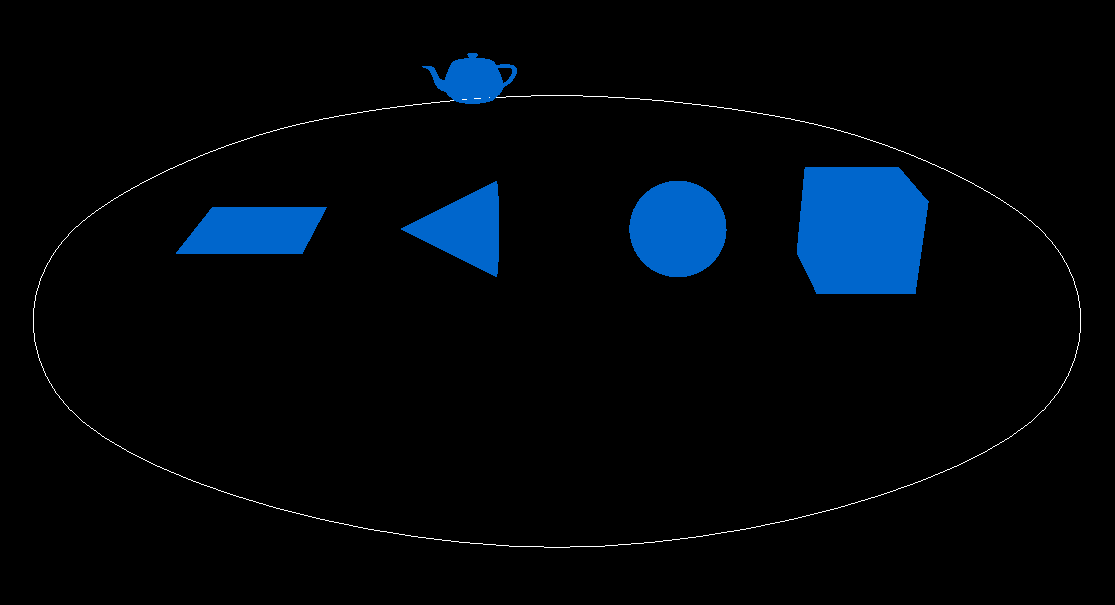
\includegraphics[scale=0.40]{primitivas} 
\caption{\label{fig:controller}Exemplo de um cenário com primitivas gráficas}
\end{figure}
\begin{lstlisting}
<scene>
    <group>
        <color G=0.4 B=0.8/>
        <translate X="25" Y="0" Z="0" />
        <scale X="2" Y="2" Z="2" />
        <models>
            <model file = "box.3d" />
        </models>
    </group>
    <group>
        <color G=0.4 B=0.8/>
        <translate X="10" Y="0" Z="0" />
        <scale X="2" Y="2" Z="2" />
        <models>
            <model file = "sphere.3d" />
        </models>
    </group>
    <group>
        <color G=0.4 B=0.8/>
        <scale X="4" Y="4" Z="4" />
        <translate X="-5" Y="0" Z="0" />
        <rotate angle="90" axisX="0" axisY="0" axisZ="1" />
        <models>
            <model file = "cone.3d" />
        </models>
    </group>
    <group>
        <color G=0.4 B=0.8/>
        <scale X="2" Y="2" Z="2" />
        <translate X="-25" Y="0" Z="0" />
        <models>
            <model file = "plane.3d" />
        </models>
    </group>
    <group>
        <color G=0.4 B=0.8/>
        <scale X="0.3" Y="0.3" Z="0.3" />
        <translate time="10" >
            <point X="0" Y="0" Z="40" />
            <point X="28.284" Y="0" Z="28.284" />
            <point X="40" Y="0" Z="0" />
            <point X="28.284" Y="0" Z="-28.284" />
            <point X="0" Y="0" Z="-40" />
            <point X="-28.2847" Y="0" Z="-28.284" />
            <point X="-40" Y="0" Z="0" />
            <point X="-28.284" Y="0" Z="28.284" />
        </translate>
        <scale X="4" Y="2" Z="2" />
        <rotate angle="-90" axisX="1" axisY="0" axisZ="0" />
        <models>
            <model file = "teapot.3d" />
        </models>
    </group>
</scene>
\end{lstlisting}
\subsection{Sistema solar dinâmico}
Nesta fase o nosso sistema solar dinâmico, todos os planetas têm o movimento de translação em redor do Sol na sua órbita respetiva, assim como
os seus próprios movimentos de rotação sobre si mesmos. Para além disso, desenhamos a óbita de um cometa que é a figura primitiva gerada com
recurso a Patches de Bézier nesta fase. Por último, também desenhamos as órbitas e movimentos das luas dos planetas.
\begin{figure}[H]
\centering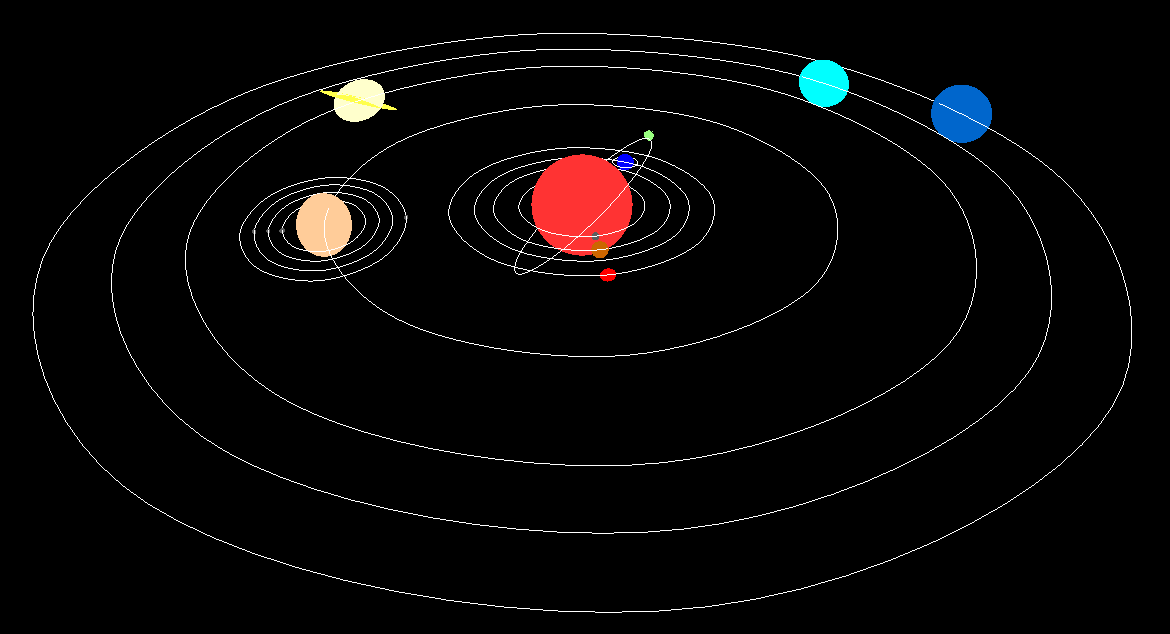
\includegraphics[scale=0.35]{ll} 
\caption{\label{fig:controller}Sistema solar dinâmico em modo fill}
\end{figure}
\begin{figure}[H]
\centering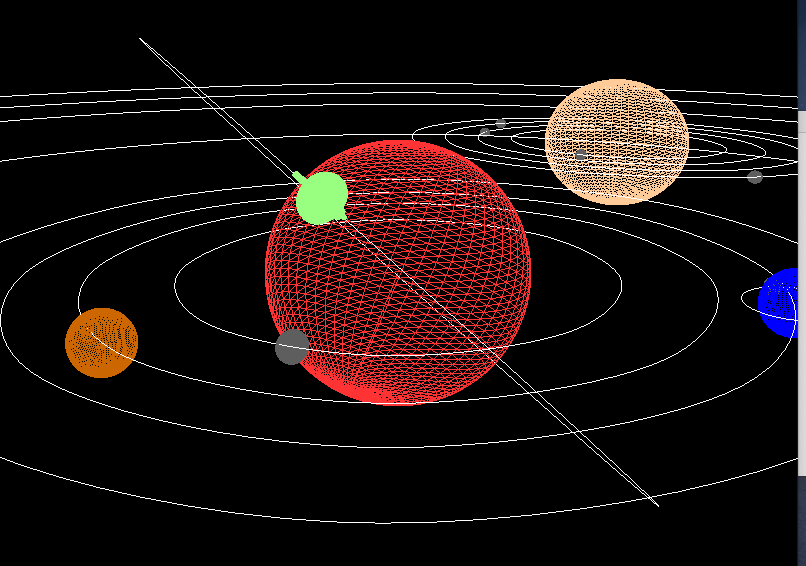
\includegraphics[scale=0.40]{lines} 
\caption{\label{fig:controller}Sistema solar dinâmico em modo lines}
\end{figure}
\begin{lstlisting}
    <scene>
	<group>
        <!-- SOL -->
		<color R=1 G=0.2 B=0.2/>
		<scale X=4 Y=4 Z=4/>
		<rotate time=10 aXisY=1/>
		<models>
			<model file=sphere.3d/>
		</models>
	</group>
	<group>
	<!--Cometa -->
		<color R=0.6 G=1.0 B=0.5 />
		<scale X=0.1 Y=0.1 Z=0.1/>
		<rotate angle=45 axisX=1 axisY=0 axisZ=0 />
		<translate time=100>
			<point X=0 Y=0 Z=15 />
			<point X=10.607 Y=0 Z=10.607 />
			<point X=15 Y=0 Z=0 />
			<point X=10.607 Y=0 Z=-10.607 />
			<point X=0 Y=0 Z=-15 />
			<point X=-10.607 Y=0 Z=-10.607 />
			<point X=-15 Y=0 Z=0 />
			<point X=-10.607 Y=0 Z=10.607 />
		</translate>
		<models>
			<model file=teapot.3d />
		</models>
	</group>
    <group>
        <!-- MERCURIO -->
		<color R=0.37 G=0.37 B=0.37/>
		<scale X=0.1 Y=0.1 Z=0.1/>
		<rotate time=10 axisY=1/>
		<translate time=15>
			<point X=10 Y=0 Z=0/>
			<point X=7.071 Y=0 Z=-7.071/>
			<point X=0 Y=0 Z=-10/>
			<point X=-7.071 Y=0 Z=-7.071/>
			<point X=-10 Y=0 Z=0/>
			<point X=-7.071 Y=0 Z=7.071/>
			<point X=0 Y=0 Z=10/>
			<point X=7.071 Y=0 Z=7.071/>
		</translate>
		<models>
			<model file=sphere.3d/>
		</models>
	</group>
    <group>
        <!-- VENUS -->
		<color R=0.8 G=0.4/>
		<scale X=0.2 Y=0.2 Z=0.2/>
		<rotate time=10 axisY=1/>
		<translate time=20>
			<point X=14 Y=0 Z=0/>
			<point X=9.899 Y=0 Z=-9.899/>
			<point X=0 Y=0 Z=-14/>
			<point X=-9.899 Y=0 Z=-9.899/>
			<point X=-14 Y=0 Z=0/>
			<point X=-9.899 Y=0 Z=9.899/>
			<point X=0 Y=0 Z=14/>
			<point X=9.899 Y=0 Z=9.899/>
		</translate>
		<models>
			<model file=sphere.3d/>
		</models>
	</group>
    <group>
        <!-- TERRA -->
		<color B=1/>
		<scale X=0.2 Y=0.2 Z=0.2/>
		<rotate time=10 axisY=1/>
		<translate time=25>
			<point X=17 Y=0 Z=0/>
			<point X=12.021 Y=0 Z=-12.021/>
			<point X=0 Y=0 Z=-17/>
			<point X=-12.021 Y=0 Z=-12.021/>
			<point X=-17 Y=0 Z=0/>
			<point X=-12.021 Y=0 Z=12.021/>
			<point X=0 Y=0 Z=17/>
			<point X=12.021 Y=0 Z=12.021/>
		</translate>
		<models>
			<model file=sphere.3d/>
		</models>
        <group>
        <!-- LUA -->
			<color R=0.37 G=0.37 B=0.37/>
			<scale X=0.15 Y=0.15 Z=0.15/>
			<rotate time=10 axisY=1/>
			<translate time=20 >
				<point X=0 Y=0 Z=3 />
				<point X=2.121 Y=0 Z=2.121 />
				<point X=3 Y=0 Z=0 />
				<point X=2.121 Y=0 Z=-2.121 />
				<point X=0 Y=0 Z=-3 />
				<point X=-2.121 Y=0 Z=-2.121 />
				<point X=-3 Y=0 Z=0 />
				<point X=-2.121 Y=0 Z=2.121 />
			</translate>
			<models>
				<model file=sphere.3d />
			</models>
		</group>
	</group>
    <group>
        <!-- MARTE -->
		<color R=1/>
		<scale X=0.15 Y=0.15 Z=0.15/>
		<rotate time=10 axisY=1/>
		<translate time=30>
			<point X=21 Y=0 Z=0/>
			<point X=14.849 Y=0 Z=-14.849/>
			<point X=0 Y=0 Z=-21/>
			<point X=-14.849 Y=0 Z=-14.849/>
			<point X=-21 Y=0 Z=0/>
			<point X=-14.849 Y=0 Z=14.849/>
			<point X=0 Y=0 Z=21/>
			<point X=14.849 Y=0 Z=14.849/>
		</translate>
		<models>
			<model file=sphere.3d/>
		</models>
	</group>
    <group>
        <!-- JUPITER -->
		<color R=1 G=0.8 B=0.6/>
        <scale X=0.5 Y=0.5 Z=0.5/>
		<rotate time=10 axisY=1/>
		<translate time=80>
			<point X=40 Y=0 Z=0/>
			<point X=28.284 Y=0 Z=-28.284/>
			<point X=0 Y=0 Z=-40/>
			<point X=-28.284 Y=0 Z=-28.284/>
			<point X=-40 Y=0 Z=0/>
			<point X=-28.284 Y=0 Z=28.284/>
			<point X=0 Y=0 Z=40/>
			<point X=28.284 Y=0 Z=28.284/>
		</translate>
		<models>
			<model file=sphere.3d/>
		</models>
		<group>
        <!-- LUA EUROPA-->
		<color R=0.37 G=0.37 B=0.37/>
        <scale X=0.04 Y=0.04 Z=0.04/>
		<translate time=10 >
			<point X=0 Y=0 Z=3 />
			<point X=2.121 Y=0 Z=2.121 />
			<point X=3 Y=0 Z=0 />
			<point X=2.121 Y=0 Z=-2.121 />
			<point X=0 Y=0 Z=-3 />
			<point X=-2.121 Y=0 Z=-2.121 />
			<point X=-3 Y=0 Z=0 />
			<point X=-2.121 Y=0 Z=2.121 />
		</translate>
		<models>
			<model file=sphere.3d/>
		</models>
		</group>
		<group>
        <!-- LUA GANIMEDES-->
		<color R=0.37 G=0.37 B=0.37/>
        <scale X=0.04 Y=0.04 Z=0.04/>
		<translate time=20 >
			<point X=0 Y=0 Z=4 />
			<point X=2.828 Y=0 Z=2.828 />
			<point X=4 Y=0 Z=0 />
			<point X=2.828 Y=0 Z=-2.828 />
			<point X=0 Y=0 Z=-4 />
			<point X=-2.828 Y=0 Z=-2.828 />
			<point X=-4 Y=0 Z=0 />
			<point X=-2.828 Y=0 Z=2.828 />
		</translate>
		<models>
			<model file=sphere.3d/>
		</models>
		</group>
		<group>
        <!-- LUA IO -->
		<color R=0.37 G=0.37 B=0.37/>
        <scale X=0.04 Y=0.04 Z=0.04/>
		<translate time=30 >
			<point X=0 Y=0 Z=5 />
			<point X=3.536 Y=0 Z=3.536 />
			<point X=5 Y=0 Z=0 />
			<point X=3.536 Y=0 Z=-3.536 />
			<point X=0 Y=0 Z=-5 />
			<point X=-3.536 Y=0 Z=-3.536 />
			<point X=-5 Y=0 Z=0 />
			<point X=-3.536 Y=0 Z=3.536 />
		</translate>
		<models>
			<model file=sphere.3d/>
		</models>
		</group>
		<group>
        <!-- LUA CALISTO -->
		<color R=0.37 G=0.37 B=0.37/>
        <scale X=0.04 Y=0.04 Z=0.04/>
		<translate time=40 >
			<point X=0 Y=0 Z=6 />
			<point X=4.242 Y=0 Z=4.242 />
			<point X=6 Y=0 Z=0 />
			<point X=4.242 Y=0 Z=-4.242 />
			<point X=0 Y=0 Z=-6 />
			<point X=-4.242 Y=0 Z=-4.242 />
			<point X=-6 Y=0 Z=0 />
			<point X=-4.242 Y=0 Z=4.242 />
		</translate>
		<models>
			<model file=sphere.3d/>
		</models>
		</group>
	</group>
    <group>
        <!-- SATURNO -->
		<color R=1 G=1 B=0.8/>
		<scale X=0.4 Y=0.4 Z=0.4/>
		<rotate time=10 axisY=1/>
		<translate time=100>
			<point X=60 Y=0 Z=0/>
			<point X=42.426 Y=0 Z=-42.426/>
			<point X=0 Y=0 Z=-60/>
			<point X=-42.426 Y=0 Z=-42.426/>
			<point X=-60 Y=0 Z=0/>
			<point X=-42.426 Y=0 Z=42.426/>
			<point X=0 Y=0 Z=60/>
			<point X=42.426 Y=0 Z=42.426/>
		</translate>
		<models>
			<model file=sphere.3d/>
		</models>
		<group>
        <!-- ANEL SATURNO -->
		<color R=1 G=1 B=0.3/>
		<scale X=1.8 Y=0.1 Z=1/>
		<rotate angle=35 axisZ=1/>
		<models>
			<model file=sphere.3d/>
		</models>
		</group>
	</group>
    <group>
        <!-- URANO -->
		<color G=1 B=1/>
		<scale X=0.35 Y=0.35 Z=0.35/>
		<rotate time=10 axisY=1/>
		<translate time=170>
			<point X=70 Y=0 Z=0/>
			<point X=49.497 Y=0 Z=-49.497/>
			<point X=0 Y=0 Z=-70/>
			<point X=-49.497 Y=0 Z=-49.497/>
			<point X=-70 Y=0 Z=0/>
			<point X=-49.497 Y=0 Z=49.497/>
			<point X=0 Y=0 Z=70/>
			<point X=49.497 Y=0 Z=49.497/>
		</translate>
		<models>
			<model file=sphere.3d/>
		</models>
	</group>
	<group>
        <!-- NEPTUNO -->
		<color G=0.4 B=0.8/>
		<scale X=0.35 Y=0.35 Z=0.35/>
		<rotate time=10 axisY=1/>
		<translate time=200>
			<point X=80 Y=0 Z=0/>
			<point X=56.569 Y=0 Z=-56.569/>
			<point X=0 Y=0 Z=-80/>
			<point X=-56.569 Y=0 Z=-56.569/>
			<point X=-80 Y=0 Z=0/>
			<point X=-56.569 Y=0 Z=56.569/>
			<point X=0 Y=0 Z=80/>
			<point X=56.569 Y=0 Z=56.569/>
		</translate>
		<models>
			<model file=sphere.3d/>
		</models>
	</group>
</scene>
\end{lstlisting}
\newpage
\section{Conclusão}
Nesta terceira fase conseguiu-se explorar as animações OpenGL baseadas em
translações e rotações, nomeadamente os conceitos associados a curvas de Catmull-Rom.
As superfícies cúbicas de Bezier permitiram a construção de primitivas
com bastante complexidade(neste projeto a primitiva escolhida foi um Teapot).
Cumpriram-se todos os objetivos propostos, apesar de algumas dificuldades
encontradas, principalmente na geração de figuras primitivas através de Patches de Bézier.
Espera-se na próxima fase, além dos requisitos já propostos, também melhorar alguns detalhes de fases anteriores.
\end{document}
